% !TEX encoding = UTF-8
% 第七章（解读）：机制排除——谱迁移、正交阻尼、滞后、clamp-free 桥
% 对应论文 §5.4（Refuting spectral migration）、§5.5（orthogonal damping
% and sensing lag）、§5.6（clamp-free bridge）；图 29、31、32，表 3。

\section{机制排除：谱迁移、正交阻尼、滞后与 clamp-free 桥}
\label{sec:ch07}

\begin{keybox}{本章速览}
\begin{itemize}
  \item 谱迁移在它唯一可能起作用的景观里也被反驳：两个方向同钉 $2/\eta$
        （$\lambda_{1}=40.1$、$\lambda_{2}=40.0$），只阻尼 $u_{1}$ $\to$
        $u_{1}$ 上逃逸（$40.1\to65.2$，seed 0）而 $\lambda_{2}$ 留在
        $39.6$——无流动；$k{=}1{:}\,64.0<k{=}2{:}\,75.2\approx
        k{=}5{:}\,77.4$——自稳定帽的逐方向结构。
  \item C4 正交阻尼：$d\in\{1,1.5,2,4,8\}$ 全部钉在 $2/\eta\approx40$
        （$0/5$ 发散）；代价是收敛变慢（loss $0.11\to0.59$）、沿 $u_{1}$
        振荡缩小（$|x_{t}|$ $0.18\to0.03$）；$d\geq4$ 时 CI 骤宽
        （$\pm9$ vs $\pm0.3$/$\pm1.7$）——G4（理论缺口之四，见
        第九章）的实测。
  \item 滞后无害、方向不准才致命：滞后但精确的 $\hat u(t-k)$
        （$k{=}1,2,3$）与 $k{=}0$ 数值相同地上逃逸到 $261.8\pm5.4$；滞后
        的更新方向传感器 $\Delta\theta_{t-k}\propto-\mathbf{g}$ 钉在
        $2/\eta$（$40.10\pm0.13$/$40.03\pm0.02$/$40.03\pm0.03$）——
        自致传感失败。
  \item clamp-free 桥：去掉 $\max(\cdot,1)$ 钳位、$100\%$ 触发仍不逃逸
        （$\lhatg=17.14\pm1.21$ vs SGD $18.73\pm1.29$，$\Delta=-1.59$
        在 CI 内；SAM $12.91\pm0.59$，差 $-5.8$）——惰性不是钳位假象。
  \item 研究日志亮点：发现 24 的``0/3000 触发''后来被发现 27 证明是自家
        钳位假象——论文把自家 bug 转化成稳健性检验的实例。
\end{itemize}
\end{keybox}

\paragraph{本章在论文中的位置。}
本章对应论文 §5.4--§5.6，兑现第 \ref{sec:ch05} 章预告的四个压力测试中的
三个（§5.5 一个小节管两个：正交阻尼与传感滞后）。每一个都堵住对秩-1 失败
的一种替代解读：``锐度搬走了''（谱迁移，§\ref{sec:ch07-migration}）；
``阻尼错了方向/传感器太旧''（正交阻尼与滞后，
§\ref{sec:ch07-orth}--\ref{sec:ch07-lag}）；``执行器根本没开火''
（clamp-free 桥，§\ref{sec:ch07-bridge}）。第四个压力测试（规模复现）
在解读第八章。合围之后，``只有全局动作能下行''的排序才算扛住了证伪。

\subsection{谱迁移反驳：在它唯一可能起作用的地方检验}
\label{sec:ch07-migration}

\paragraph{逻辑。}
帽移除说预言：特征向量之间\emph{没有流动}——阻尼 $u_{1}$ 只会让 $u_{1}$
自己失去帽而上逃逸，别的方向不受影响。替代的``谱迁移''
（spectral migration）读法把锐度当作某种守恒预算：阻尼一个方向，锐度应
\emph{搬}到未阻尼的方向。这个读法要成立，前提是存在第二个尖方向可搬。第
\ref{sec:ch05} 章的默认景观是 1-D sharp
（$\lambda_{1}=261.8\pm5.4\gg\lambda_{2}\approx0.6$，图
\ref{fig:ch05-rankk}）——迁移在那里无处着力。所以论文构造了一个迁移
\emph{唯一可能起作用}的景观：多输出各向同性 teacher--student（``各向同性''
即各方向性质相同、无偏好方向——构造出的合成教师在多个方向有对称的
尖锐度，好比人为造出两条等深峡谷，用来测试锐度会不会搬家），其 EoS 谱把
两个方向同时钉在 $2/\eta$：$\lambda_{1}=40.1$、$\lambda_{2}=40.0$。

\paragraph{检验与观测。}
只阻尼 $u_{1}$（秩-1、精确特征向量）。迁移读法的预言：$\lambda_{2}$ 应
升过 $2/\eta$，吸收``守恒的锐度预算''。实际观测（论文图 29）：$u_{1}$
上逃逸（$40.1\to65.2$，seed 0 轨迹示例）而 $\lambda_{2}$ \emph{留在 $39.6$}——
没有流动，且 $\lmax>2/\eta$。迁移被反驳。

\begin{figure}[!ht]
\centering
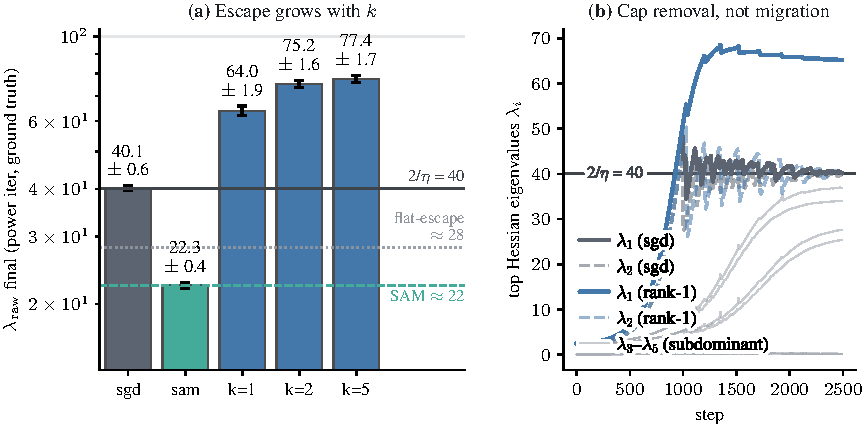
\includegraphics[width=0.95\linewidth]{29_multisharp_migration.pdf}
\caption{多尖锐景观测试（论文图 29；$n{=}5$ 种子）。构造的多输出各向同性
teacher--student 把\emph{两个}方向钉在 $2/\eta$（$\lambda_{1}=40.1$、
$\lambda_{2}=40.0$）。左：只阻尼 $u_{1}$（秩-1）让 $u_{1}$ 上逃逸而
$\lambda_{2}$ 保持钉住——无流动，在迁移貌似可行的地方反驳迁移。右：
$k>1$ 此时起作用，揭示自稳定帽的逐方向结构（数值见正文）。}
\label{fig:ch07-multisharp}
\end{figure}

\paragraph{$k$ 在这里起作用——帽的逐方向结构。}
与 1-D 情形的 $k$-不变（$k{=}1,2,5,10$ 逐 bit 相同）不同，多尖锐景观中
$k$ 有意义：$k{=}1{:}\,64.0<k{=}2{:}\,75.2\approx k{=}5{:}\,77.4$。机制
：每阻尼一个坐在 EoS 帽上的方向 $=$ 移除一个帽 $=$ 该方向独立上逃逸——
$k$ 越大，逃逸的方向越多，$\lmax$ 越高。这反过来确认了帽是\emph{逐方向}（per-direction）
的自治结构：$u_{1}$ 的帽被移除并不连带解除 $u_{2}$ 的帽。顺带一提，多尖锐
景观的上逃逸（$64.0$--$77.4$）远低于 1-D 景观的 $261.8\pm5.4$——每个
方向的曲率质量有限，逃逸有界。

\paragraph{研究日志中的演进。}
日志里这是``option B''：发现 23 在 1-D 景观推翻迁移后，遗留问题是
``$\lambda_{1}\approx\lambda_{2}$ 时迁移是否显形''；发现 25 构造了多尖锐
景观并给出否定答案，论文的理论节（自稳定帽机制）就此定案。数字以论文为
准。

\subsection{C4 正交阻尼：对称控制以对称的方式失败}
\label{sec:ch07-orth}

\paragraph{设计。}
秩-1 plant 阻尼 top 方向；C4（正交阻尼，orthogonal damping，阻尼顶部
方向之外的\emph{全部}正交补——与顶部特征向量垂直的所有参数方向构成
的空间）是对称控制——阻尼\emph{其余一切}：
\begin{equation}
  \Delta\theta=-\eta\left(\mathbf{g}_{\parallel}+\mathbf{g}_{\perp}/d\right),
  \label{eq:ch07-orth}
\end{equation}
保持 top 方向梯度 $\mathbf{g}_{\parallel}$ 原封不动。论文理论节的推论给
出干净预言（$x$-递推指位移变量 $x$ 的迭代式、$y^{*}$ 指均衡时
尖锐度超出阈值 $2/\eta$ 的量——二维状态变量的定义见第九章）：
$\mathbf{g}_{\parallel}$ 保持 $\Rightarrow$ $x$-递推就是无
阻尼的 Damian 映射 $\Rightarrow$ $y^{*}=0$——top 方向的自稳定不受触碰
。

\paragraph{结果：全 $d$ 钉住。}
扫 $d\in\{1,1.5,2,4,8\}$（$n{=}5$，MLP 全批）：$\lmax$ 全部钉在
$2/\eta\approx40$——$40.2,\,40.3,\,38.9,\,43.4,\,40.1$；每个 $d$ 下
$0/5$ 种子发散。

\paragraph{代价与次级现象。}
其一，收敛变慢：最终 loss 从 $0.11$ 升到 $0.59$（$d\to8$）。其二，沿
$u_{1}$ 的振荡缩小：$|x_{t}|$ 从 $0.18$ 降到 $0.03$——补集被冻结后振荡
幅度反而更小，但帽不降。其三，$d\geq4$ 时逐种子散布骤宽：CI $\pm9$
（$d{=}4$）vs $\pm0.3$（$d\leq1.5$）、$\pm1.7$（$d{=}2$）。原因：冻结
补集移走了帮助界定 $u_{1}$ 振荡的方向，常数-$\alpha$ 的 2-D 约简（假设渐进尖锐化系数 $\alpha$ 在窗口内恒定的二维约化，见第九章）失去精度
——这是论文理论 gap \textbf{G4}（缺口之四：二维约化缺少四次及更高阶
景观项、无法给振荡幅度 $|x|$ 定界，见第九章）的实测实例，不是逃逸
（每个 $d$ 下 $0/5$
发散）。

\paragraph{与秩-1 的对照：反向夹逼。}
两个单方向控制以\emph{相反}的机制失败：top 阻尼把帽向上移除（上逃逸过
$2/\eta$，体制 (ii)）；补集阻尼把帽原地留下（钉在 $2/\eta$）。一个向上
、一个不动，都不下逃逸——两个方向一夹，帽的不可下行性得到确认。

\subsection{滞后 vs 方向不准：把混杂变量拆开}
\label{sec:ch07-lag}

\paragraph{混杂。}
第 \ref{sec:ch05} 章体制 (i) 用的延迟更新传感器
$\hat v_{k}=\Delta\theta_{t-k}/\|\cdot\|$ 把两件事混在一起：
\emph{滞后}（信息旧 $k$ 步）与\emph{用错方向}（用更新/梯度方向而非特征
向量）。拆开检验（$n{=}5$，MLP）：

\paragraph{臂 1：滞后但精确——滞后无害。}
传感器 $\hat v_{k}=\hat u(t-k)$（$k{=}1,2,3$；$\hat u$ 为精确的幂迭代
估计，只是旧 $k$ 步）。结果：与 $k{=}0$ \emph{数值相同}地上逃逸到
$261.8\pm5.4$。原因：$u_{1}$ 在慢的 $O(1/\eta)$ 时间尺度上旋转
（即要约 $1/\eta$ 步才明显变化），
$\hat u(t-k)\approx u_{1}(t)$——帽仍被移除。滞后本身无害。

\paragraph{臂 2：滞后且用更新方向——自致传感失败。}
传感器 $\hat v_{k}=\Delta\theta_{t-k}\propto-\mathbf{g}$
（$k{=}1,2,3$）。结果：钉在 $2/\eta$——$40.10\pm0.13$、
$40.03\pm0.02$、$40.03\pm0.03$。起作用的原因不是陈旧而是
\textbf{自致传感失败}（self-induced sensing failure，执行器自己的动作把传感器转离目标方向）：plant 自己的阻尼把更新方向转离 $u_{1}$，执行器随之
脱开。体制 (i) 的根源是\emph{方向不准}，不是滞后。

\paragraph{病理对照：无钳位的执行器病态。}
去掉钳位后，陈旧的瑞利商翻 $\gamma<0$（$\gamma=1-1/d$ 为阻尼强度，
见第九章）、变成反向阻尼（负阻尼——不压制
反而放大振荡）——$k{=}1$ 时在步
$\sim540$ 发散。注意这个发散正是 §\ref{sec:ch07-bridge} clamp-free 语义
精读的对照物：那里的符号翻转被截断、有界；这里的原始因子随陈旧瑞利商
塌缩 $\gamma\to-\infty$、无界。

\begin{figure}[!ht]
\centering
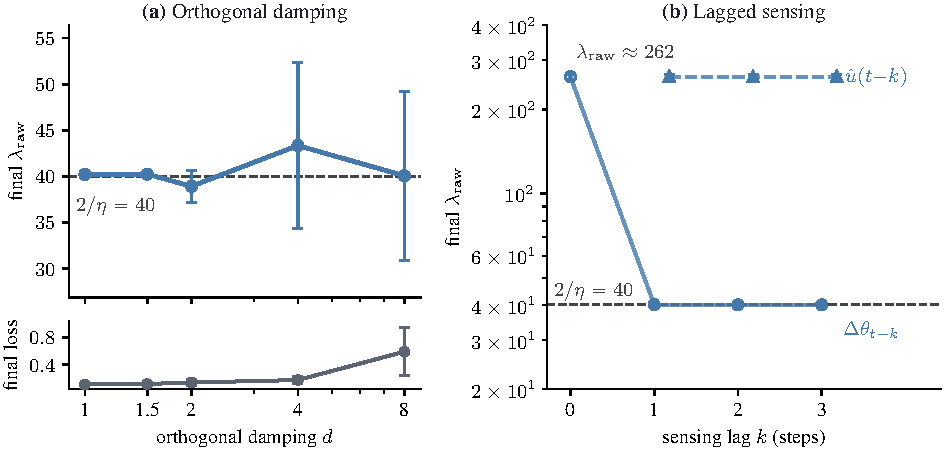
\includegraphics[width=0.95\linewidth]{31_c4_lagged_controls.pdf}
\caption{MLP 全批设置上的两个进一步控制（论文图 31；$n{=}5$ 种子）。
(a) 正交阻尼（C4）：每个 $d\in\{1,\dots,8\}$ 下 $\lmax$ 钉在
$2/\eta\approx40$（$0/5$ 发散；loss 从 $0.11$ 升到 $0.59$，右轴）——
阻尼补集碰不到 top 方向的帽。(b) 滞后 vs 不准：滞后但精确的传感器
$\hat u(t-k)$ 上逃逸到 $261.8\pm5.4$（$\triangle$），与 $k{=}0$ 相同；
滞后的更新方向传感器 $\Delta\theta_{t-k}$ 钉在 $2/\eta$（$\circ$）。
滞后无害；钉住的是梯度方向代理，不是陈旧。}
\label{fig:ch07-c4lag}
\end{figure}

\paragraph{小结。}
帽对传感\emph{滞后}稳健、对传感\emph{不准}不稳健——体制 (i) 的归因由
``旧''改为``偏''。

\subsection{clamp-free 桥：惰性不是钳位假象}
\label{sec:ch07-bridge}

\paragraph{动机：自家门控的嫌疑。}
第 \ref{sec:ch06} 章的 X-SAM 消融给论文自家门控出了一道难题：clamped
X-SAM 的秩-1 修正 $0\%$ 步触发，而 faithful 每步触发——$\max(\cdot,1)$
钳位可以制造休眠（dormant）。而 at-scale 秩-1 plant 用的是\emph{同一个}
钳位，其``惰性''判定（触发比例 $\le4\%$、$\approx$SGD）部分是基于这个
观察作出的——它也因此沾上了同样的嫌疑：也许真正中和它的是钳位、不是景观
。桥接臂正面回：同一 CIFAR-100/ResNet-18 设置、确定性 CUDA、$n{=}5$ 种子、
\texttt{-{}-no-clamp}——无 $\max(\cdot,1)$ 门、每个方向每步都触发
（触发比例 $100\%$）、原始除数 $d=\hat\lambda/\lambda_{\mathrm{targ}}$
允许低于 $1$。

\paragraph{clamp-free 语义精读：不是``总是阻尼''臂。}
编辑（对梯度的手工改写）为 $\mathbf{g}\mapsto\mathbf{g}-f\,\alpha\,\hat v$（其中
$\alpha=\langle\mathbf{g},\hat v\rangle$；$f$ 即编辑因子——对梯度沿
$\hat v$ 分量的改写强度系数），$f=1-1/d$ \emph{截断到}
$[-1,1)$：
\begin{itemize}
  \item $\hat\lambda>\lambda_{\mathrm{targ}}$（$d>1$）：$f\in(0,1)$，
        编辑是阻尼，$\hat v$ 分量留下 $\alpha/d$；
  \item $\hat\lambda<\lambda_{\mathrm{targ}}$（$d<1$）：$f<0$，符号
        翻转——编辑不反对反而\emph{增强} $\hat v$ 分量：有界的反向增强
        （bounded sign-flip anti-damping）；
  \item 截断保证编辑幅度 $\le|\alpha|$、编辑后的 $\hat v$ 分量
        $\le2|\alpha|$——反向增强有界、不会爆炸。
\end{itemize}
与 §\ref{sec:ch07-lag} 的无截断滞后 plant 对比：那里的原始因子随陈旧
瑞利商塌缩 $\gamma\to-\infty$，无界反向阻尼，$k{=}1$ 步 $\sim540$ 发散
；这里符号翻转被截断。\textbf{``是界而不是门''}（门 = 只在条件满足时
才让干预发生；界 = 干预每步都发生、但幅度被截断在固定区间内）把两个
clamp-free 陈述
分开——它们一致而不矛盾。

\paragraph{桥接结果（论文表 3）。}
晚期（步 $\geq2000$）单 HVP 梯度瑞利商 $\lhatg$，确定性 512 样本评估批
，$n{=}5$ 种子，mean$\pm95\%$ CI：

\begin{table}[!ht]
\centering\small
\caption{clamp-free 桥，CIFAR-100/ResNet-18、确定性 CUDA（$n{=}5$ 种子
）：晚期（步 $\geq2000$）$\lhatg$ mean$\pm95\%$ CI 与秩-1 修正的触发比例
（对应论文表 3）。\textbf{仅协议内比较}：$\lhatg$ 是固定评估批上的单 HVP
下界代理，其绝对尺度（13--18）与 at-scale 控制的 ARPACK $\lmax$ 尺度
（22--29）不可比。}
\label{tab:ch07-bridge}
\begin{tabular}{lcc}
\toprule
臂 & 晚期 $\lhatg$ & 触发比例 \\
\midrule
SGD & $18.73\pm1.29$ & --- \\
秩-1（clamped C3） & $18.13\pm1.47$ & $4\%$ \\
\textbf{秩-1（clamp-free C3）} & $\mathbf{17.14\pm1.21}$ & $100\%$ \\
SAM & $12.91\pm0.59$ & --- \\
\bottomrule
\end{tabular}
\end{table}

\paragraph{读数。}
其一，clamp-free 臂\emph{不上逃逸}：与 SGD 差 $\Delta=-1.59$、与
clamped 臂差 $-0.99$——差值量级与两臂 CI 半宽（$1.2$--$1.5$）相当、
区间互相重叠，按第~\ref{sec:ch03-stats}~节的判读规则读作``检测不到
差异''，远不到 MLP 精确
$\vtope$ plant 的上逃逸量级（第 \ref{sec:ch05} 章的 $261.8\pm5.4$）。
其二，clamp-free 比 SGD 低 $\sim1.6$——方向与 Duan 等 (2026) 的预测
一致，但量级远小于 SAM 的 $-5.8$ 且在 CI 内，``贡献可忽略''的裁决不变
。其三，同一驱动重验确定性三向：SAM（$12.91\pm0.59$）低于两个秩-1 臂
且 CI 不重叠——at-scale 排序在 X-SAM 消融引入的更严确定性标准下依然成立。

\paragraph{为何报 $\lhatg$ 而非 ARPACK $\lmax$（within-protocol（协议内——只在同一测量协议之内比较）警告）。}
做桥接实验时，幂迭代 $\lmax$ 估计尚不可信——伪收敛问题后来才在规模实验
（§5.7，解读第八章）中诊断。因此论文报告确定性的 per-model 代理
$\lhatg$（$\lmax$ 的下界代理），所有比较在协议内进行；$\lhatg$ 尺度
（13--18）与 ARPACK $\lmax$ 尺度（22--29）\emph{不可比}——跨协议读数是
本章最容易犯的错误。

\begin{figure}[!htbp]
\centering
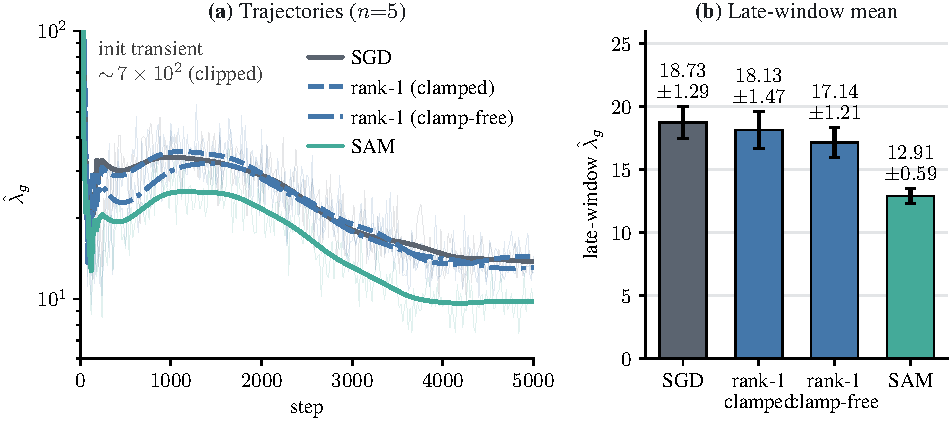
\includegraphics[width=0.92\linewidth]{32_bridge_clampfree_c3.pdf}
\caption{clamp-free 桥（论文图 32；确定性 CUDA，$n{=}5$ 种子）：SGD、
clamped 秩-1、clamp-free 秩-1 与 SAM 的晚期 $\lhatg$
（mean$\pm95\%$ CI；臂用线型与颜色区分，灰度打印下仍可分辨）。
(a) 为对数域高斯平滑后的轨迹（淡细线为未平滑均值，初始瞬态两采样保留未平滑）。
clamp-free 臂每步都触发，却仍在 SGD 与 clamped 臂的 CI 内——无上逃逸、
无钳位假象——而 SAM 以不重叠的 CI 坐在下方。}
\label{fig:ch07-bridge}
\end{figure}

\paragraph{结论：惰性稳健地独立成立。}
对 at-scale 秩-1 结果的两个残余可疑读数——钳位假象与休眠传感器——被
\emph{分别}排除：惰性在去掉钳位（$100\%$ 触发仍不逃逸，
图 \ref{fig:ch07-bridge}）后成立，也在修复传感器（true-$\lmax$ plant：
无钳位地板、ARPACK 传感、全力开火，仍与 sharpness 无关——``有动作仍被
钉住''，详见解读第八章）后成立。

\subsection{研究日志中的演进：一次自我纠错}
\label{sec:ch07-log}

日志里，发现 24（X-SAM 消融第一版）曾断言``rank-1 修正 $0/3000$ 步触发
、结构性死代码''。发现 27 在取得 Duan 等 (2026) 的精确算法（Eq.~11）后
发现：该断言是\emph{自家钳位}（$\max(\cdot,1)$ 自门控）制造的假象——
faithful 版每步触发（$100\%$）。论文吸收了这次纠错：§5.3 改为忠实四臂
对比（第 \ref{sec:ch06} 章），本节的 clamp-free 桥正是把自家的测量伪迹
转化为对 at-scale 判定的稳健性检验。方法论启示：可疑的阴性结果要先排除
``自家仪器造成的休眠''再下结论——而排除的办法，就是把怀疑对象本身变成实验
臂。

\subsection*{本章要点}
\begin{itemize}
  \item \textbf{谱迁移被反驳}：即使在两个方向同钉 $2/\eta$
        （$\lambda_{1}=40.1$、$\lambda_{2}=40.0$）的多尖锐景观，阻尼
        $u_{1}$ 只让 $u_{1}$ 上逃逸（$40.1\to65.2$）、$\lambda_{2}$ 原地
        不动（$39.6$）；$k$ 的作用
        （$k{=}1{:}\,64.0<k{=}2{:}\,75.2\approx k{=}5{:}\,77.4$）揭示帽的
        逐方向结构。
  \item \textbf{C4 正交阻尼}全 $d\in\{1,1.5,2,4,8\}$ 钉在 $2/\eta\approx
        40$（$0/5$ 发散），代价是收敛变慢（loss $0.11\to0.59$）、振荡
        缩小（$|x_{t}|$ $0.18\to0.03$）；$d\geq4$ 时 CI 骤宽（$\pm9$）
        是 G4 的实测——两个单方向控制反向夹逼，都不下逃逸。
  \item \textbf{滞后无害、方向不准致命}：$\hat u(t-k)$ 与 $k{}=0$ 同样
        上逃逸到 $261.8\pm5.4$（$u_{1}$ 在慢 $O(1/\eta)$ 尺度旋转）；
        $\Delta\theta_{t-k}\propto-\mathbf{g}$ 钉在 $2/\eta$
        （$40.10\pm0.13$/$40.03\pm0.02$/$40.03\pm0.03$）——体制 (i) 的
        根源是自致传感失败；无钳位时陈旧瑞利商翻 $\gamma<0$、$k{=}1$ 步
        $\sim540$ 发散。
  \item \textbf{clamp-free 桥}：$100\%$ 触发仍不逃逸
        （$\Delta=-1.59$ vs SGD，在 $\sim1.5$ 单位 CI 内；SAM 的 $-5.8$
        才是真实降幅）；``是界而不是门''把有界反向增强与无截断发散分开
        ；$\lhatg$ 尺度（13--18）与 ARPACK 尺度（22--29）不可比。
  \item \textbf{四个压力测试合围}：单方向控制的失败不是迁移、不是阻尼
        错边、不是传感器太旧、不是钳位休眠——``只有全局动作能下行''的
        排序依然成立；研究日志中``0/3000 触发 $\to$ 自家钳位假象''的纠错
        （发现 24 $\to$ 27）是论文自我纠错的方法论亮点。
\end{itemize}
